\textit{Escherichia coli} is among the most widely studied organisms, and the species is very diverse\cite{Lukjancenko2010, Selander1987}.
%In addition to being a member of the human gut microbiome, \textit{E. coli} are found in soil, water, and livestock. The majority of lineages are harmless, but some can cause serious illness.  Thus, detecting and identifying the different lineages has remained
Because of this diversity, many methods have been developed to differentiate the different  \textit{E. coli} lineages.  In 1987, Selandar  and colleagues used electrophoretic analysis of a 35 enzyme digest to classify the \textit{E. coli} Reference Collection (ECOR) in 6 phylogenetic groups (A-F)\cite{Selander1987}.  Clermont and colleagues published their triplex PCR method\cite{Clermont2000} of phylotyping, which proved to be an extremely valuable tool to differentiate groups A, B1, B2, and D, being cited over 625 times as of April 2018.  In 2013, Clermont and colleagues published an update to this work\cite{Clermont2013}, in which they showed that adding a 4th set of primers achieved higher resolution by expanded the method to detect groups E, F; additional primers were identified to differentiate the cryptic clades.  This approach has been widely adopted as the method is reliable, easy to interpret, can correctly classify about 95\% of \textit{E. coli} strains, and can be performed rapidly.

Other typing schemes have been developed to classify \textit{E. coli} strains. These include the Achtman 7 gene Multi Locus Sequence Typing (MLST)\cite{Achtman2012, Alikhan2018}, Michigan EcMLST\cite{Qi2004}, whole-genome MLST (\url{http://www.applied-maths.com/applications/wgmlst}), core-genome MLST\cite{DeBeen2015}, two-locus MLST\cite{Weissman2012}, and ribosomal MLST\cite{Jolley2012}. All these sequencing-based methods classify \textit{E. coli} with greater accuracy and granularity than PCR-based phylotyping, but at the cost of simplicity: in addition to not requiring seqeuncing, it is easier to discuss a small set of phylotypes compared to the results of typing methods aimed at capturing greater genomic diversity. As a result, the Clermont 2013 phylotyping scheme remains a popular tool for \textit{E. coli} classification.

We developed EzClermont to provide a simple in silico implementation of the Clermont phylotyping algorithm for genome assemblies. We have implemented the software as a web application and as a command-line tool for those needing to process large numbers of assemblies.

In short, the software uses regular expressions to perform an in silico PCR, determining a phylotype according to the presence or absence of the alleles. As assemblies may contain alleles interrupted by breaks between contigs, we give the user the option to allow partial matches (ie, if one of the two primers matched, but the expected position of the other primer fell beyond the sequence end).

To assess the performance of EzClermont, we selected training,  test, and validation datasets.  Additionally, the strains from Clermont, 2013 Figure 1 are used as unit tests in the package.

As PCR primers do not necessarily need 100\% sequence homology to function, we determined the variability at the priming sites across a large set of  strains. To do this, we downloaded a training set of 523 genome assemblies from NCBI Bioprojects PRJNA218110\cite{lindsey_multiplex_2017}, PRJNA231221\cite{sichtig_fdaargos_2019}, and PRJNA352562.  These sequences were selected to gain a broad overview of the genomic diversity in \textit{E. coli}. From each assembly, we extracted the 7 regions matching the theoretical amplicons of the quadriplex, E-specific, C-specific, and E/C control primer sets from Clermont 2013.  Any differences between an assemblies sequence and the Clermont primer sequence were incorporated into the search query in a manner akin to degenerate primer design. Differences occuring in the last 5 nucleotides on the 3’ regions were not incorporated, as those can be used to differentiate alleles \cite{Stadhouders2010}.


The test set consisted of the strains listed in Sims and Kim 2011\cite{Sims2011} (Table S1), and the validation set of 95 strains was the genomes from Clermont 2015\cite{Denamur2015} (Table S2)\footnote{6 of the 101 total strains were omitted as no genome assembly was available.}.  Comparing the reported phylogroup and the EzClermont phylogroup for the 19 strains in Sims and Kim (excluding strains reported in both studies),  3 of the 19 did not agree (Table \ref{tab:sims}). Two of those (IAI39, SMS-3-5) have been shown by other works to have the phylotype that EzClermont predicted. The one strain that typed differently (APEC01) was examined and was found to have the ArpA allele not normally detected in B2 strains. It unclear why this allele is not detected by traditional methods.



\begin{table}[h]
\centering
\caption{Comparing EzClermont to phylotypes reported by Sims and Kim 2011\cite{Sims2011}}
\label{tab:sims}
\begin{tabular}{llccl}
  Strain  & Assembly         & Sims and Kim & EzClermont & Notes                                        \\
  \hline
APEC01  & GCA\_003028815.1 & B2           & A          & found arpA fragment                          \\
IAI39   & GCA\_000026345.1 & D            & F          & See Hazen 2017\cite{Hazen2017}; reported as phylogroup F     \\
SMS-3-5 & GCA\_000019645.1 & D            & F          & See Vangchhia 2016\cite{Vangchhia2016}; reported as phylogroup F
\end{tabular}
\end{table}

We ran EzClermont on the 95 strains from Clermont, et al 2015 and compared the results to the reported phylotype; 89 of the 95 strains classifications matched.  To determine whether the inconsistent phylogroup assignments matched phylogeny, we then generated a parsimony tree using kSNP3\cite{Gardner2015a}, and plotted with ggtree\cite{Yu2017a}. This revealed that the EzClermont classification of ECOR46 (similar IAI39 and SMS-3-5) appears to match the true phylogeny, as opposed to the phylogroup reported in the literature (Figure \ref{fig:cladogram}).  Of the remaining isolates that did not match, all detected at least one theoretical amplicon that was not reported to be there (Table S3). Further, a wide application of EzClermont by Zhou et al.\cite{zhou_users_2019} to representative \textit{E. coli}  strains in Enterobase was largely in agreement with both higher-resolution sequence typing and with ClermonTyping\cite{beghain_clermontyping:_2018}, another in silico tool for detecting Clermont types.


\begin{figure}[h]
  \centering
  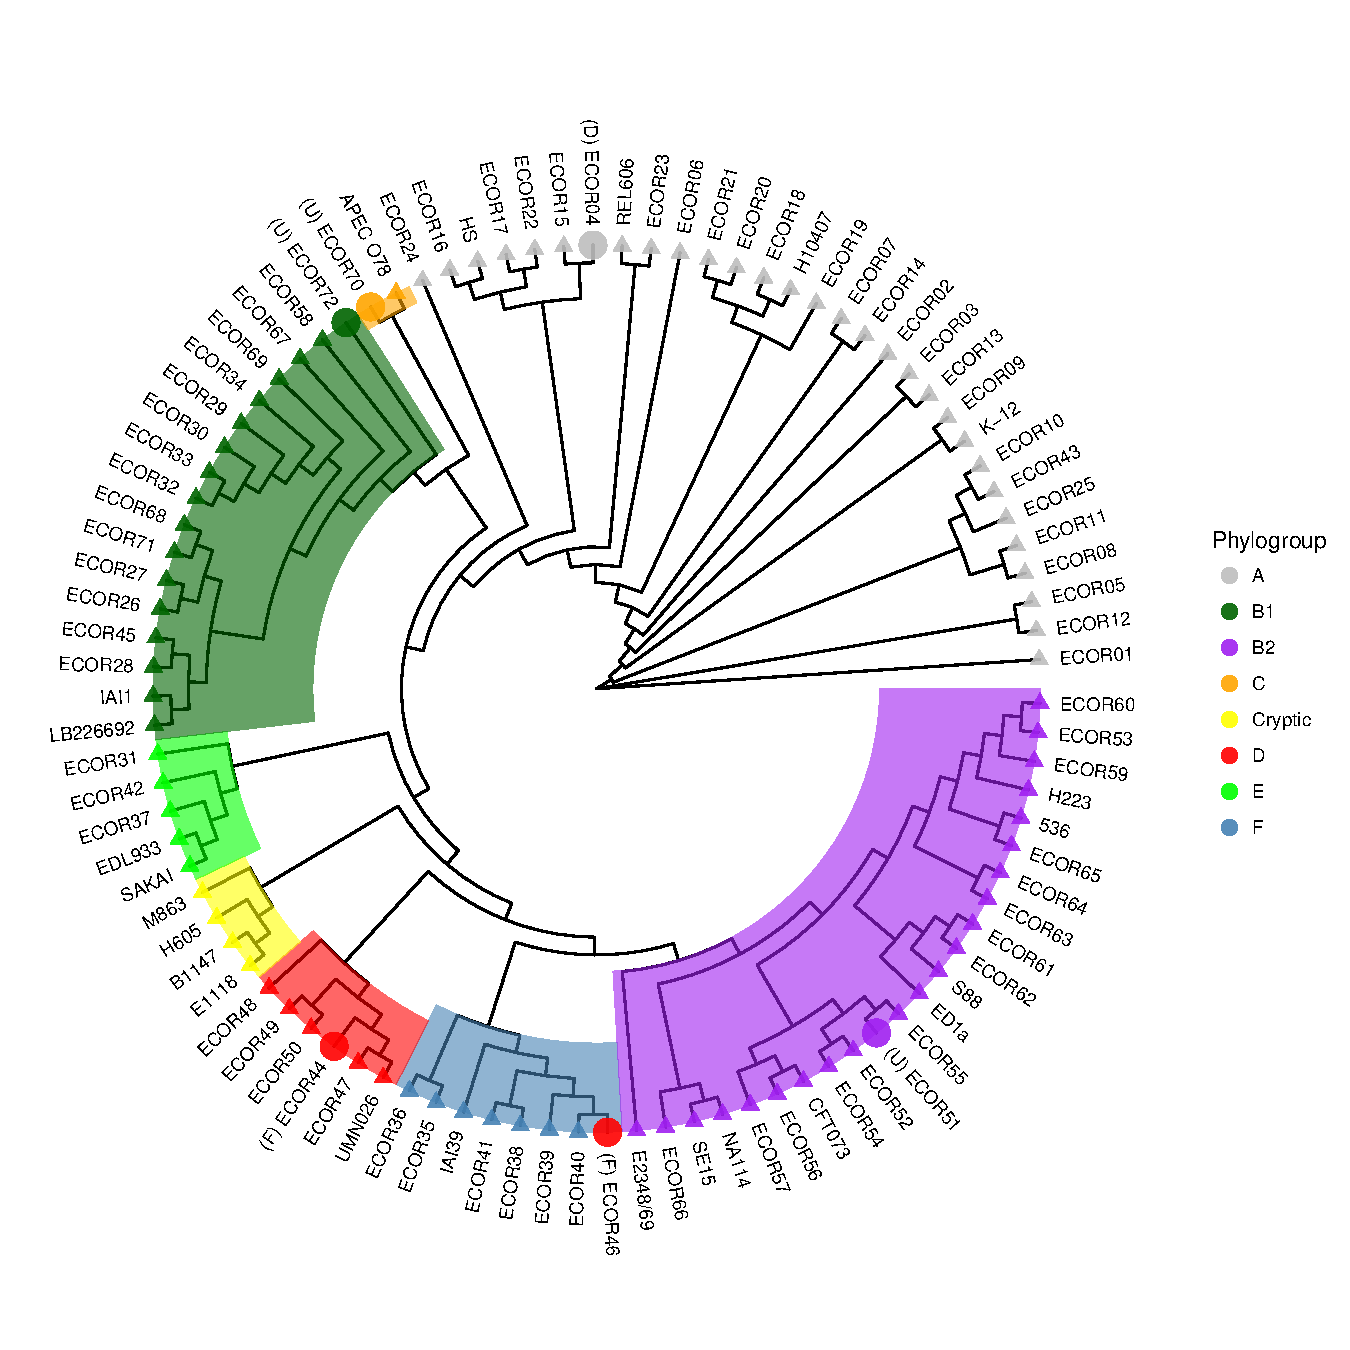
\includegraphics[width=.5\textwidth]{./analysis/cladogram.pdf}
  \caption{ Parsimony cladogram of strains from Clermont et al 2015. Tree was generated with kSNP3 (k=19). Enlarged circular tips show where EzClermont differed from reported phylogroup (EzClermont type show in brackets).}
  \label{fig:cladogram}
\end{figure}


Considering both the testing and validation datasets (114 strains), EzClermont has an accuracy of 94\%. Given the ease of use of the web app for simple queries, its incorporation into Enterobase, and the standalone speed of execution for larger batches, we hope that EzClermont will be of continued use to the scientific community.
